\documentclass{beamer}
% \documentclass[notes]{beamer}

\usepackage{graphicx}       % Extended support for \includegraphics
\usepackage{tikz}           % Powerful drawing package, part of pgf
\usepackage{url}            % \url command for decent line breaks in urls
\usepackage{array}          % Improved array support
\usepackage{textcomp}       % Extra symbols

% Enable this for summary printout
% \usepackage{pgfpages}\pgfpagesuselayout{4 on 1}[
%     a4paper, landscape, border shrink=2mm]


\usetikzlibrary{matrix}             % Grid placement
\usetikzlibrary{positioning}        % Anchor placement support
\usetikzlibrary{calc}               % Coordinate calculations
\usetikzlibrary{shapes.geometric}   % cylinder
\usetikzlibrary{shapes.symbols}     % cloud
\usetikzlibrary{shapes.arrows}      % arrow shapes
\usetikzlibrary{shapes.multipart}
\usetikzlibrary{fit}                % Fitting outline to shape
\usetikzlibrary{shadows}
\usetikzlibrary{arrows}
\usetikzlibrary{chains}

% Common TikZ definitions
\tikzset{
    % This seems a reasonably comfortable arrow shape
    >=stealth,
%
    % Used for creating an exact fit to an existing list of objects
    tight fit/.style={fit=#1, inner sep=0, line width=0},
%
    % Draws a reasonably sensible looking disk icon
    disk icon/.style={
        draw, thick, cylinder, shape border rotate=90,
        minimum width=1cm, minimum height=.75cm},
%
    % A moderate highlighting fill
    background fill/.style={fill=black!15},
    % A gentle highlighing fill
    highlight fill/.style={fill=green!60!blue!20},
    % A rather darker fill for shadows
    shadow fill/.style={fill=gray}}

% It's handy to have a foreground and background layer available.
\pgfdeclarelayer{background}
\pgfdeclarelayer{foreground}
\pgfsetlayers{background,main,foreground}


\usetheme{dlstalk}
\setbeamertemplate{navigation symbols}{}
\setbeamertemplate{items}[circle]

\hyphenpenalty 4000 \sloppy

% \title{A new Fast Data Logger and Viewer at Diamond:\\the FA Archiver}
\title[Fast Feedback]{A Technical Description of\\Fast Feedback}
\author{Michael Abbott}
\date{Software Developers Away Day\\ 12th February 2015}




\begin{document}


\begin{frame}
\titlepage
\end{frame}

% Place date discreetely on every slide.
\setbeamertemplate{footline}{\hspace*{\fill}\insertdate}


% ------------------------------------------------------------------------------
%
\begin{frame}\frametitle{Fast Orbit Feedback}

The purpose of Fast Orbit Feedback is to stabilise the electron beam so that the
optical beam delivered to beamlines does not move too much.

\medskip

Current target is to limit motion to $\pm 3\%$ beam size for frequencies up to
100\,Hz.

\medskip

Higher frequency motion enlarges the beam seen by users and is not controllable
by the current feedback implementation.

\end{frame}


% ------------------------------------------------------------------------------
%
\begin{frame}\frametitle{Impact of Orbit Feedback by Frequency}
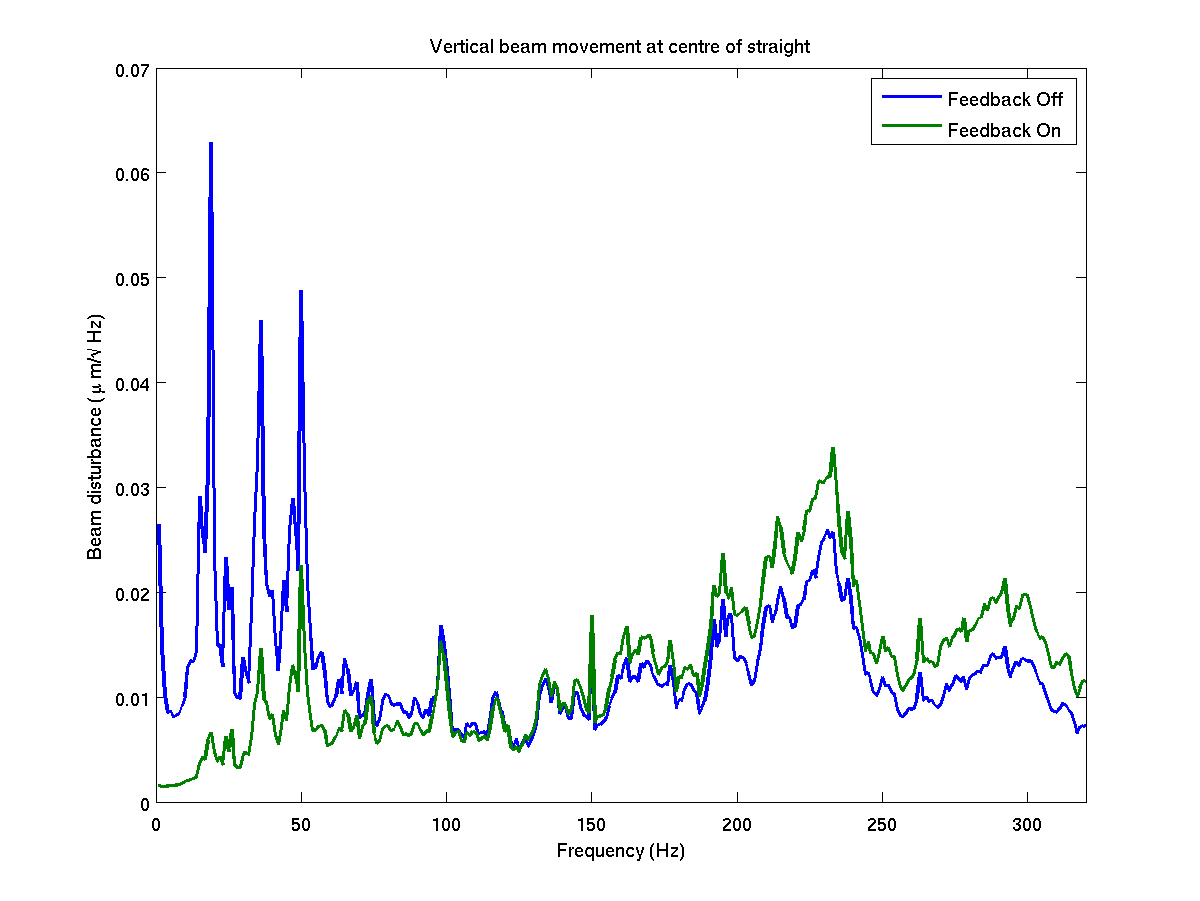
\includegraphics[width=\linewidth]{fb-on-off}
\end{frame}


% ------------------------------------------------------------------------------
%
\begin{frame}\frametitle{Integrated Impact of Orbit Feedback}
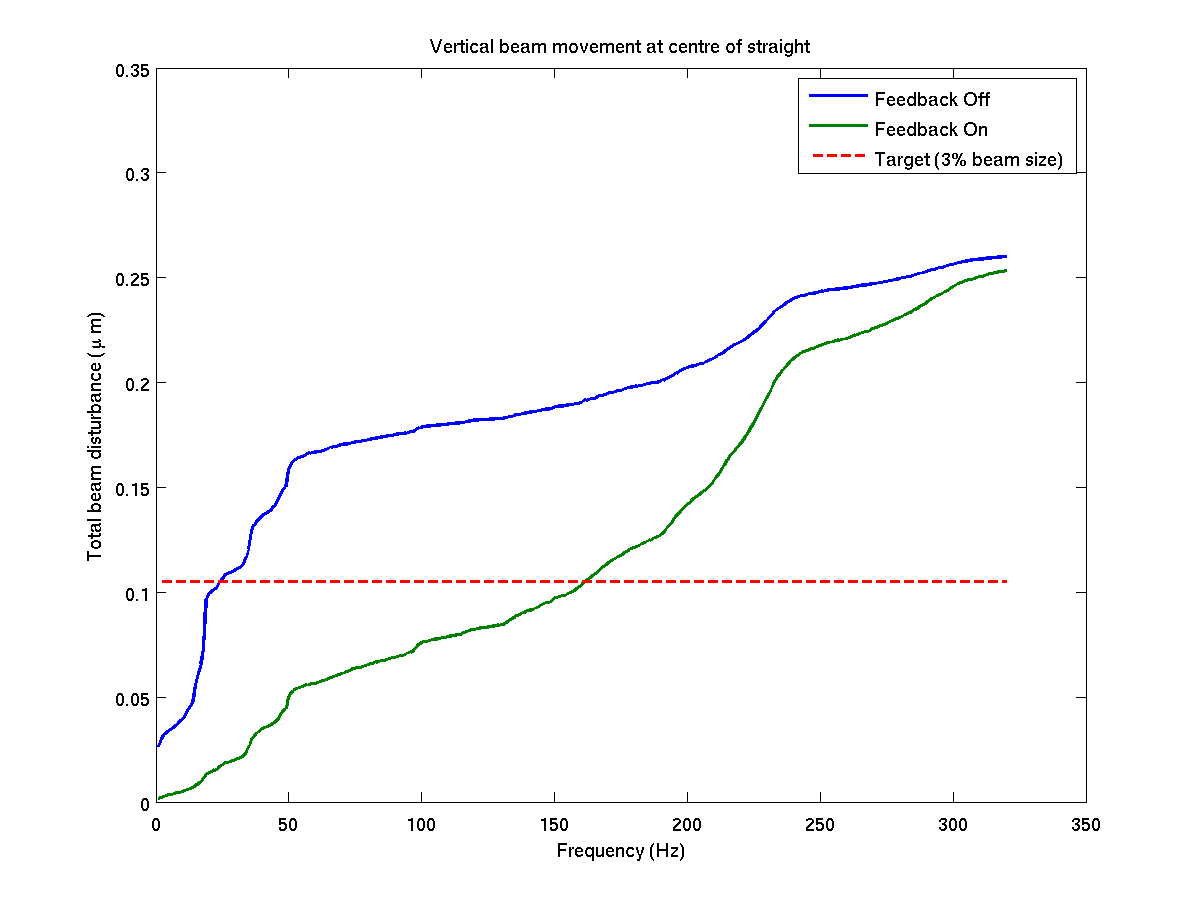
\includegraphics[width=\linewidth]{fb-on-off-integ}
\end{frame}


% ------------------------------------------------------------------------------
%
\begin{frame}\frametitle{Feedback Signal Processing}

172 beam position monitors are used to control 344 corrector magnets:

\begin{itemize}
\item 500\,MHz signal picked up from beam by 172 button blocks
\item Signal sampled at 117\,MHz (32\,MHz intermediate frequency)
\item Signal filtered down to 10\,kHz signal and $X,Y$ computed
\item Position communicated to each of 24 feedback processors
\item Position error used to compute magnet correction
\item Correction communicated to each of 344 power supply controllers
\item Power supply drives correction coils in focusing magnets
\item Beam is steered back into position
\end{itemize}

\end{frame}


% ------------------------------------------------------------------------------
%
\begin{frame}\frametitle{Electron Beam Fast Feedback}
\begin{center}
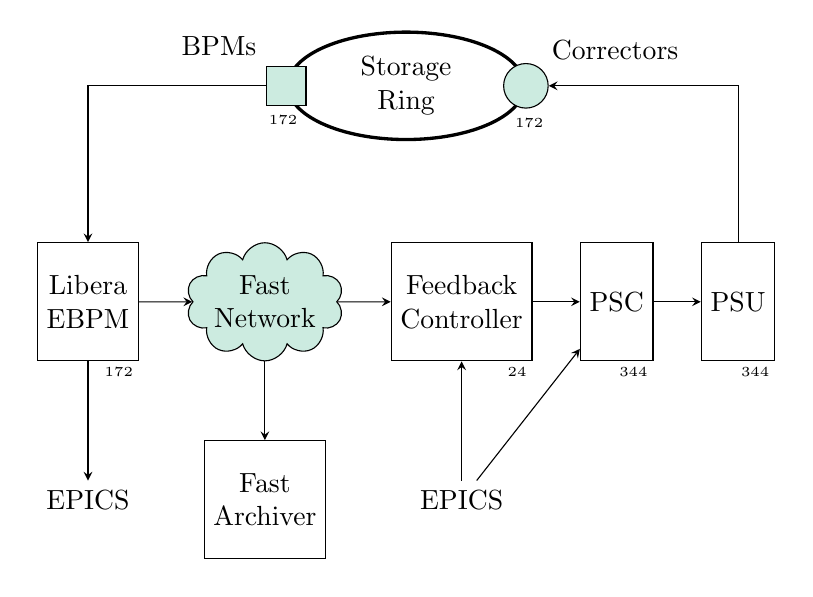
\begin{tikzpicture}

\tikzset{every node/.style={align=center}}

\node (sr) [draw, ellipse, very thick, minimum width=30mm]
    {Storage\\Ring};
\node (bpm) [draw, rectangle, highlight fill, inner sep=2.5mm,
    label={above left:BPMs},
    label={below:\tiny 172~}] at (sr.west) {};
\node (mag) [draw, circle, highlight fill, inner sep=2mm,
    label={above right:Correctors},
    label={below:\tiny ~172}] at (sr.east) {};

\matrix [minimum height=15mm, column sep=6mm, row sep=10mm] at (0,-40mm) {
    \node (libera) [draw, rectangle] {Libera\\EBPM}; &
    \node (cc) [draw, cloud, aspect=2, highlight fill, inner sep=0pt]
        {Fast\\Network}; &
    \node (ff) [draw, rectangle] {Feedback\\Controller}; &
    \node (psc) [draw, rectangle] {PSC}; &
    \node (psu) [draw, rectangle] {PSU};
\\
    \node (epics1) [minimum height=0] {EPICS}; &
    \node (fa) [draw, rectangle] {Fast\\Archiver}; &
    \node (epics2) [minimum height=0] {EPICS};
\\
};

\node [anchor=north east, inner sep=2pt] at (libera.south east) {\tiny 172};
\node [anchor=north east, inner sep=2pt] at (ff.south east) {\tiny 24};
\node [anchor=north east, inner sep=2pt] at (psc.south east) {\tiny 344};
\node [anchor=north east, inner sep=2pt] at (psu.south east) {\tiny 344};


\draw [->] (bpm) -| (libera);
\draw [->] (libera) -- (cc);
\draw [->] (cc) -- (ff);
\draw [->] (ff) -- (psc);
\draw [->] (psc) -- (psu);
\draw [->] (psu) |- (mag);

\draw [->] (libera) -- (epics1);
\draw [->] (cc) -- (fa);
\draw [->] (epics2) -- (ff);
\draw [->] (epics2) -- (psc);

\end{tikzpicture}

% vim: set filetype=tex:

\end{center}
\end{frame}


% ------------------------------------------------------------------------------
%
\begin{frame}\frametitle{A Quick Detailed Look}

We'll now take a quick detailed look at three corners of this system:

\begin{itemize}
\item Communication controller.
\item Feedback controller.
\item Fast Archiver.
\end{itemize}

\end{frame}


% ------------------------------------------------------------------------------
%
\begin{frame}\frametitle{Communication Controller}

\begin{itemize}

\item
The challenge: to communicate 172 beam position $X, Y$ pairs to 24 feedback
controllers every 100\,\textmu s.

\item
The technology: fiber optical connections runnng at 1\,Gbit per second
connecting all Beam Position Monitors and Feedback Controllers in a complex
redundant network.

\item
The algorithm:

\begin{enumerate}
\item At the start of every tick every BPM sends its position to all of its
neighbours.
\item Every node in the network forwards a copy of every \emph{new} position it
receives.
\item After around 45\,\textmu s every node has seen every position update.
\end{enumerate}

\end{itemize}

\end{frame}


% ------------------------------------------------------------------------------
%
\begin{frame}\frametitle{Communication Controller Network Topology}
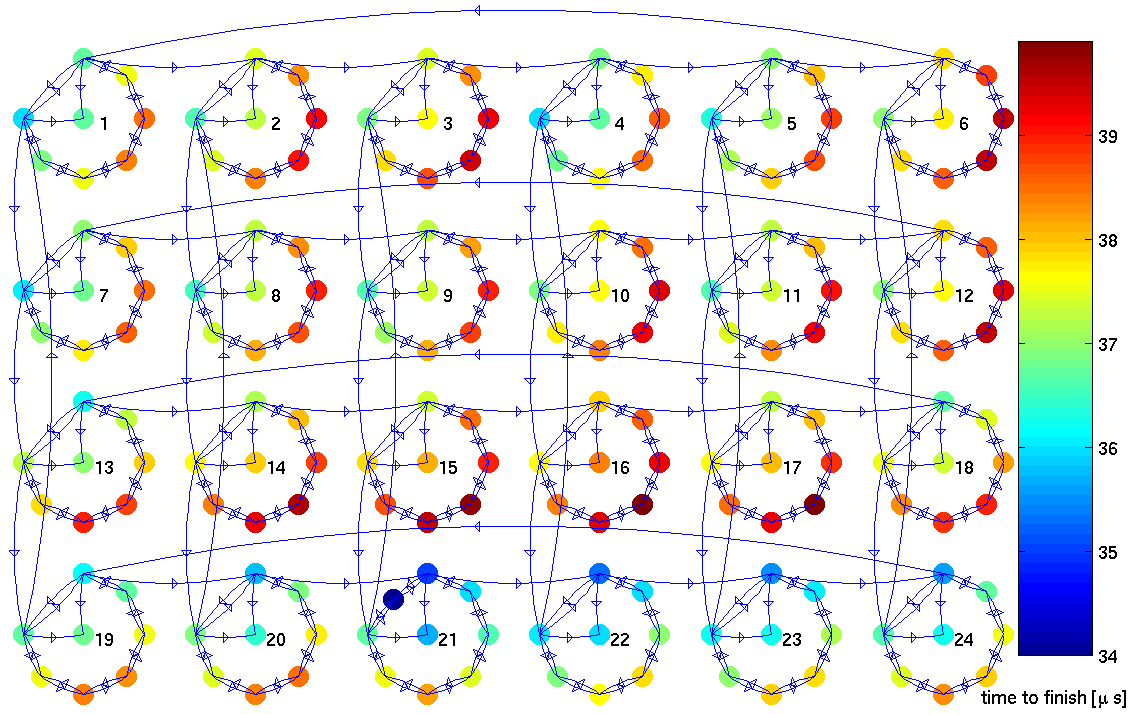
\includegraphics[width=\linewidth]{fofb}
\end{frame}



% ------------------------------------------------------------------------------
%
\begin{frame}\frametitle{Communication Controller Internals}

The Communication Controller is entirely implemented in FPGA in VHDL.

\medskip

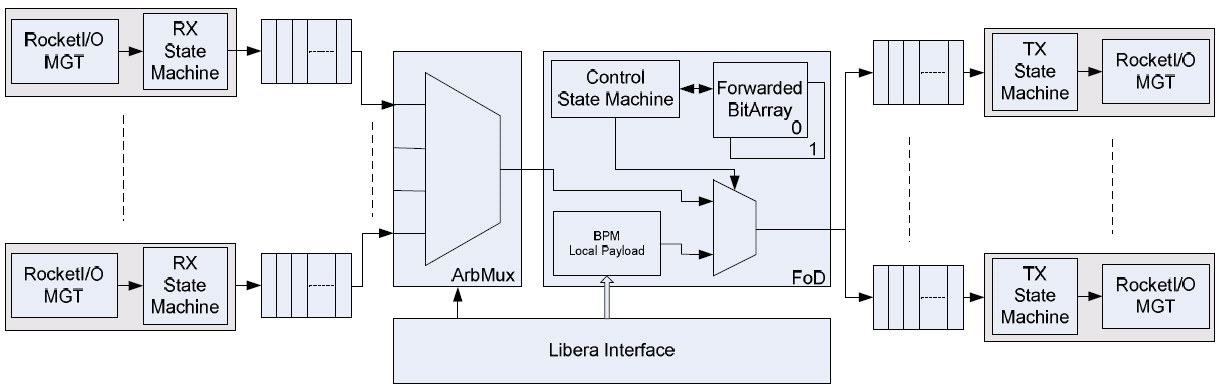
\includegraphics[width=\linewidth]{cc-internal}

\medskip

One challenge: if the internal queues overflow then data can be delayed or lost.

\end{frame}


% ------------------------------------------------------------------------------
%
\begin{frame}\frametitle{Fast Feedback Controller}

There are 24 feedback controllers, one per storage ring sector, each controlling
14 corrector magnets.  Each controller runs on a VME PowerPC processor card with
the following hardware connections:

\begin{itemize}
\item Connection to Communication Controller network through PCI Mezzanine Card
(PMC) over PCI bus.
\item Connection to Power Supply Controllers over VME backplane and optical
fibre.
\item Ethernet connection to controls network for EPICS control and status
monitoring.
\end{itemize}


\end{frame}


% ------------------------------------------------------------------------------
%
\begin{frame}\frametitle{Fast Feedback Processing}

Feedback control is performed by the following steps:

\begin{enumerate}
\item Receive interrupt from Communication Controller PMC notifying that a
complete set of BPM positions has arrived.
\item Initiate DMA from CC card to processor memory.  Takes 60\,\textmu s!
\item Convert global orbit error into local corrector error.  This is a $14
\times 172$ matrix multiplication converting 172 $X,Y$ positions into 7 $X,Y$
corrector adjustments.
\item Filter corrector error adjustment to manage spectral response and
stability.  This step involves quite a bit of control theory.
\item Sanity check correction and halt feedback if any error is found.
\item Send corrector magnet update to power supply controllers.
\end{enumerate}

\end{frame}


% ------------------------------------------------------------------------------
%
\begin{frame}\frametitle{Feedback and Timing}

The time budget for the feedback process is quite interesting.  There is a
total delay from beam measurement to correction of around 700\,\textmu s.  This
limits our bandwidth to little more than 100\,Hz.  The following are
contributions to delay:

\begin{description}
\item[150\,\textmu s] Filtering in BPM.  A natural consequence of the
100\,\textmu s update rate.
\item[45\,\textmu s] Communication from BPM to CC PMC.
\item[50\,\textmu s] DMA from CC PMC to processor RAM.
\item[40\,\textmu s] Feedback algorithm.
\item[400\,\textmu s] Power supply control.  This will be investigated...
\end{description}

\medskip

Note that little more than 10\% of the delay is spent in computation: vectorised
floating point arithmetic can be \emph{fast}!

\end{frame}


% ------------------------------------------------------------------------------
%
\begin{frame}\frametitle{The Fast Acquisition Archiver}

The nature of the Fast Feedback Communication network makes it very easy to add
nodes.  The Fast Archiver is one such node.

\medskip

The Fast Archiver captures $X,Y$ position data from BPMs at 10\,kHz, maintains a
rolling historical record, and rebroadcasts the complete data stream to all
interested parties.

\begin{itemize}

\item 256 $X,Y$ position updates every 100\,\textmu s, sustained data
rate of 20\,MB/s.

\item A fortnight of data is archived onto a dedicated 30TB server.

\item Any number of clients (limited by network connection to archive server)
can read the archive and subscribe to the rebroadcast live data stream.

\end{itemize}
\end{frame}



% ------------------------------------------------------------------------------
%
\begin{frame}\frametitle{FA Archiver in Context}
\begin{center}
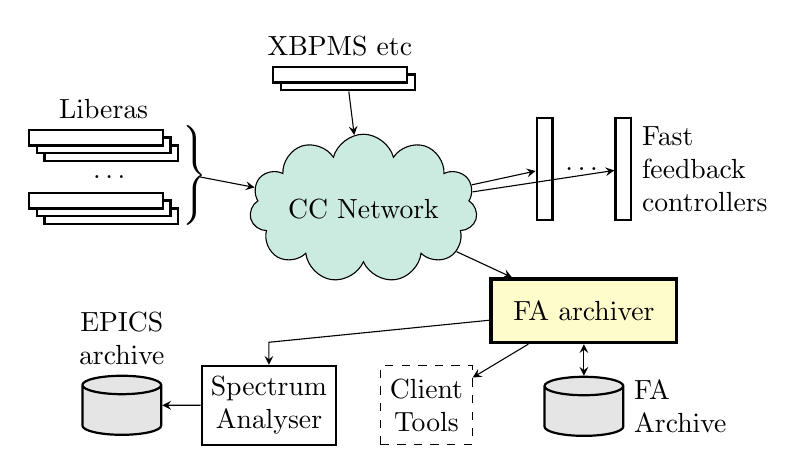
\begin{tikzpicture}

% Nice puffy cloud representing the FA network
\path[xshift=27mm, yshift=5mm, thin]
    node[draw, cloud, aspect=2, cloud puffs=11, inner sep=0pt, highlight fill]
        (fa network) {CC Network};

% Draw a stack of rectangles representing the liberas
\path[xshift=-5mm, yshift=12mm,
    libera/.style={
        draw, rectangle, thick, fill=white, inner sep=0,
        minimum width=1.7cm, minimum height=2mm}]

    { [current point is local=true]
    node[libera] {}
    ++(-1mm,1mm) node[libera] {}
    ++(-1mm,1mm) node[libera] (top libera) {}
    }

    +(0mm,-3mm) node {\dots}
    ++(0mm,-8mm)
    { [current point is local=true]
    node[libera] (bottom libera) {}
    ++(-1mm,1mm) node[libera] {}
    ++(-1mm,1mm) node[libera] {}
    }
    node[tight fit=(top libera) (bottom libera),
        right delimiter=\}, label=north:Liberas] (liberas) {};

\draw[->] ($(liberas.east)+(2.6mm,0)$) -- (fa network);

\path[xshift=25mm, yshift=21mm,
    libera/.style={
        draw, rectangle, thick, fill=white, inner sep=0,
        minimum width=1.7cm, minimum height=2mm}]

    node[libera] (xbpms) {}
    ++(-1mm,1mm) node[libera, label=north:XBPMS etc] {};

\draw[->] (xbpms) -- (fa network);


% Fast feedback controllers
\path[xshift=50mm, yshift=10mm,
    controller/.style={
        draw, rectangle, thick, inner sep=0,
        minimum width=2mm, minimum height=13mm}]

    node[controller] (left controller) {}
    ++(5mm,0mm) node {\dots}
    ++(5mm,0mm) node[controller,
        label={[align=left]right:Fast\\feedback\\controllers}]
    (right controller) {};

\draw[->] (fa network) -- (left controller);
\draw[->] (fa network) -- (right controller);

% The archiver saving into the archive store
\path[xshift=5.5cm, yshift=-8mm]
    node[draw, very thick, rectangle, inner sep=8pt, fill=yellow!20]
        (archiver) {FA archiver}

    node[disk icon, below=4mm of archiver, fill=black!10] (fa archive) {}
    node[tight fit=(fa archive),
        label={[align=left]right:FA\\Archive}] {}
    [draw,<->] (archiver) -- (fa archive);

\draw[->] (fa network) -- (archiver);

% Spectrum analyser saving into EPICS archive
\path[xshift=15mm, yshift=-20mm]
    node[draw, thick, rectangle, align=center, minimum height=10mm]
        (spectrum) {Spectrum\\Analyser}

    node[disk icon, anchor=shape center, fill=black!10,
        label={[align=center]above:EPICS\\archive}]
        (epics archive) at ($(spectrum.west)-(10mm,0)$) {}
    node[tight fit=(epics archive)] (epics archive fit) {}

    [draw,->] (spectrum) -- (epics archive fit);

\draw[->] (archiver) -- ($(spectrum)+(0,8mm)$) -- (spectrum);

% Client tools
\path[xshift=35mm, yshift=-20mm]
    node[draw, rectangle, align=center, minimum height=10mm, dashed]
        (client tools) {Client\\Tools};

\draw[->] (archiver) -- (client tools);

\end{tikzpicture}

% vim: set filetype=tex:

\end{center}
\end{frame}



% ------------------------------------------------------------------------------
%
\begin{frame}\frametitle{The Fast Acquisition Archiver}
\begin{center}
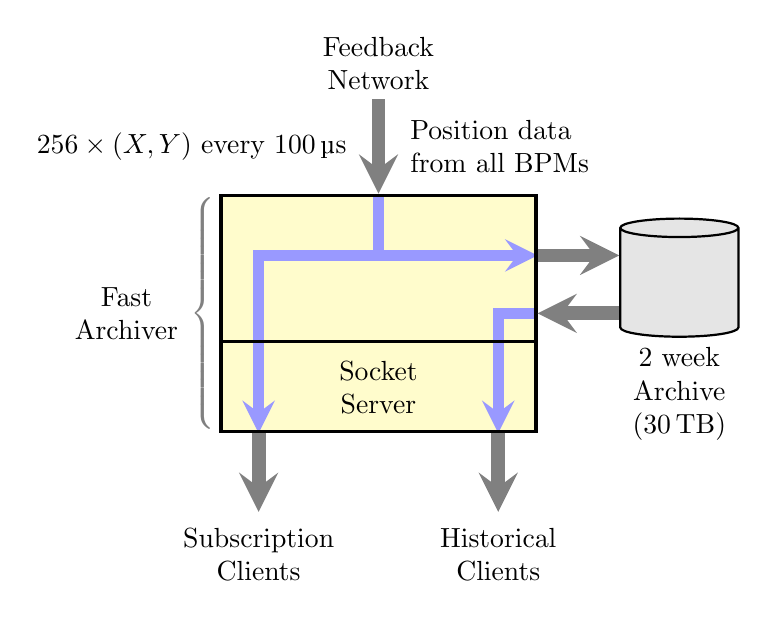
\begin{tikzpicture}

\tikzset{
    accent/.style={color=blue!40, line width=4pt},
    highlight/.style={fill=yellow!20},
    every node/.style={align=center}}

\path (0,0)
    node (cc) {Feedback\\Network}
    [draw, line width=5pt, gray, ->] (cc.south) -- ++(0,-12mm)
    coordinate (input)
    node [midway, left, black, xshift=-2mm]
        {$256\times(X,Y)$  every 100\,\textmu{}s}
    node [midway, right, black, align=left, xshift=2mm]
        {Position data\\from all BPMs};
\node (archiver) [
        draw, very thick, rectangle, anchor=north,
        label={[xshift=-4mm]left:Fast\\Archiver},
        minimum width=40mm, minimum height=30mm] at (input) {};
\path [gray] node [fit=(archiver), inner sep=0pt, left delimiter=\{] {};

\draw[very thick] (archiver.-10) -- (archiver.-170);
\path (archiver.-10) -- (archiver.south west)
    node [midway] {Socket\\Server};

\draw [line width=5pt, gray, ->] (archiver.-135) -- +(0, -10mm)
    node [black, anchor=north] {Subscription\\Clients};
\draw [line width=5pt, gray, ->] (archiver.-45) -- +(0, -10mm)
    node [black, anchor=north] {Historical\\Clients};

\begin{pgfonlayer}{background}
\path[highlight] (archiver.north west) rectangle (archiver.south east);
\draw[accent, ->] (archiver.north) |- (archiver.20);
\draw[accent, ->] (archiver.0) -| (archiver.-45);
\draw[accent, ->] (archiver.north |- archiver.20) -| (archiver.-135);
\end{pgfonlayer}

\node (disk) [disk icon, fill=black!10,
    minimum height=15mm, minimum width=15mm, xshift=18mm,
    label={below:2 week\\Archive\\(30\,TB)}]
    at (archiver.10) {};
\draw [line width=5pt, color=gray, ->]
    (archiver.20) -- (archiver.20 -| disk.west);
\draw [line width=5pt, color=gray, <-]
    (archiver.0) -- (archiver.0 -| disk.west);

\end{tikzpicture}

% vim: set filetype=tex:

\end{center}
\end{frame}



% ------------------------------------------------------------------------------
%
\begin{frame}\frametitle{FA Archiver Architecture}

\begin{itemize}

\item Very regular data feed: fixed size updates at fixed intervals.
Makes archiver design much simpler than an EPICS archiver.

\item The historical archive is fixed length, determined by disk size.  Old data
is discarded as new data arrives.

\item Data is reordered for fast read access before storage to disk.

\item File system overhead is avoided by storing archiver database on raw block
device!

\item Overview data (decimated by binning) also stored.

\item Archive indexed by timestamp of arrival of CC data.

\end{itemize}
\end{frame}



% ------------------------------------------------------------------------------
%
\begin{frame}\frametitle{FA Archiver Architecture}
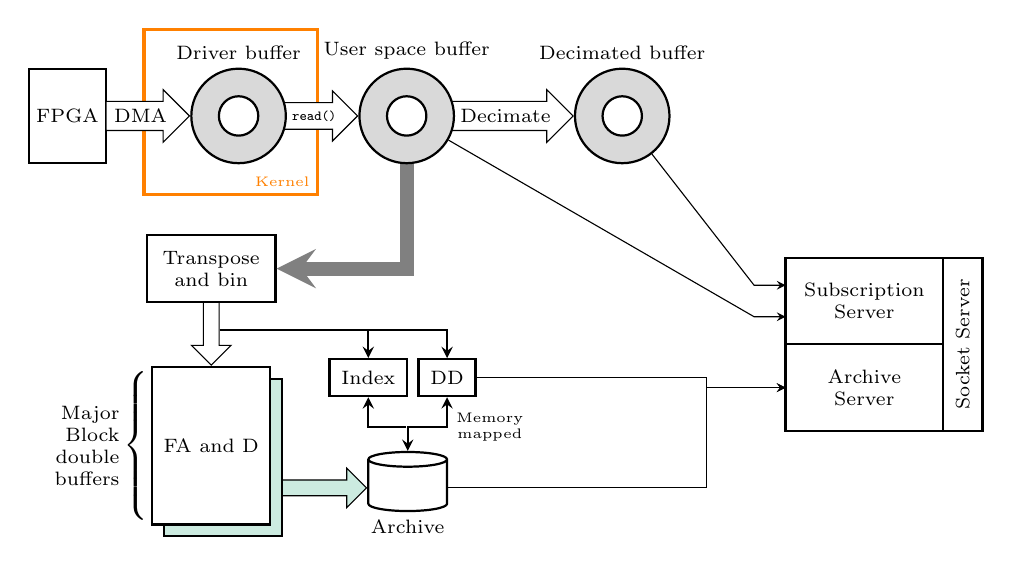
\begin{tikzpicture}[
    single arrow head extend=1.5mm]
\scriptsize

% Draws a circular buffer with name #1 east of #2 with top label #3 and centre
% label #4
\newcommand{\buffer}[3]{
\begin{pgfonlayer}{foreground}
\path
    node [draw, thick, circle, background fill,
        minimum width=12mm, anchor=west,
        label={above:#3}] (#1) at (#2.east) {}
    node [draw, thick, fill=white, circle, minimum width=5mm] at (#1) {};
\end{pgfonlayer}
}

% Sniffer device and its connections
\node [draw, thick, anchor=west, minimum height=12mm] (fpga) {FPGA};
\node [draw, single arrow, anchor=west, fill=white]
    (dma) at ($(fpga.east)-(0.2mm,0)$) {DMA};

% Device driver
\buffer{device buffer}{dma}{Driver buffer}
\node [draw, single arrow, anchor=west, fill=white]
    at ($(device buffer.east)-(0.4mm,0)$)
    (device) {\tiny\texttt{read()}};

\begin{pgfonlayer}{background}
\draw [orange, very thick] ($(device buffer)+(-12mm,11mm)$)
    rectangle ($(device buffer)+(10mm,-10mm)$);
\node [orange, anchor=south east, font=\tiny]
    at ($(device buffer)+(10mm,-10mm)$) {Kernel};
\end{pgfonlayer}


% Central raw circular buffer and decimated buffer
\buffer{raw buffer}{device}{User space buffer}
\node [draw, single arrow, anchor=west] at ($(raw buffer.east)-(0.4mm,0)$)
    (decimate) {Decimate};
\buffer{decimated buffer}{decimate}{Decimated buffer}


% Transposing to in-memory disk buffer
\node [draw, thick, anchor=north west, inner sep=2mm, align=center]
    at (15mm, -15mm)
    (transpose) {Transpose\\and bin};
\path [draw, line width=5pt, color=gray, ->] (raw buffer) |- (transpose);
\node [draw, single arrow, rotate=-90, anchor=west, minimum height=8mm]
    (transpose arrow) at ($(transpose.south)+(0,0.2mm)$) {};
\begin{pgfonlayer}{foreground}
\node [draw, thick, fill=white,
    minimum height=20mm, minimum width=15mm, anchor=north, align=center,
    left delimiter=\{, copy shadow={
        shadow xshift=1.5mm, shadow yshift=-1.5mm, highlight fill},
    label={[align=right, xshift=-3mm]left:Major\\Block\\double\\buffers}]
    (major block) at (transpose arrow.east) {FA and D};
\end{pgfonlayer}


% Archive on disk and in memory
\node [draw, single arrow, anchor=west, minimum width=1mm, minimum height=12mm,
    highlight fill]
    (archive arrow) at (major block.325) {};
\node [disk icon, anchor=west, label={below:Archive}]
    (archive) at (archive arrow.east) {};

\node [draw, thick, inner sep=1.5mm]
    (index) at ($(archive)+(-5mm,14mm)$) {Index};
\node [draw, thick, inner sep=1.5mm] (dd) at ($(archive)+(+5mm,14mm)$) {DD};

\draw [->, thick] (transpose arrow) -| (index);
\draw [->, thick] (transpose arrow) -| (dd);
\node [inner sep=0pt, line width=0] (via) at ($(archive.north)+(0,3mm)$) {};
\draw [<-, thick] (index) |- (via);
\draw [<->, thick] (dd) |- (via.center) -- (archive);

\node [right=5mm of via, align=center, font=\tiny] {Memory\\mapped};


% Socket Server
\path [draw, thick]
    (\linewidth, -40mm) rectangle ++(-5mm,22mm) coordinate (a)
    node [rotate=90, pos=0.5] {Socket Server}
    rectangle ++(-20mm,-11mm) coordinate (b)
    node [pos=0.5, align=center] {Subscription\\Server}
    rectangle ++(20mm,-11mm) coordinate (c)
    node [pos=0.5, align=center] {Archive\\Server}
    node [tight fit=(a) (b), align=center] (subscription server) {}
    node [tight fit=(b) (c), align=center] (archive server) {};

\draw [<-] ($(subscription server.west)+(0,-2mm)$)
    -- +(-4mm,0) -- (raw buffer);
\draw [<-] ($(subscription server.west)+(0,2mm)$)
    -- +(-4mm,0) -- (decimated buffer);
\draw [<-] (archive server.west) -- +(-10mm,0) |- (archive);
\draw [<-] (archive server.west) -- +(-10mm,0) |- (dd);


\end{tikzpicture}

% vim: filetype=tex:

\end{frame}


% ------------------------------------------------------------------------------
%
\begin{frame}\frametitle{Binned Archive Data}
\begin{center}
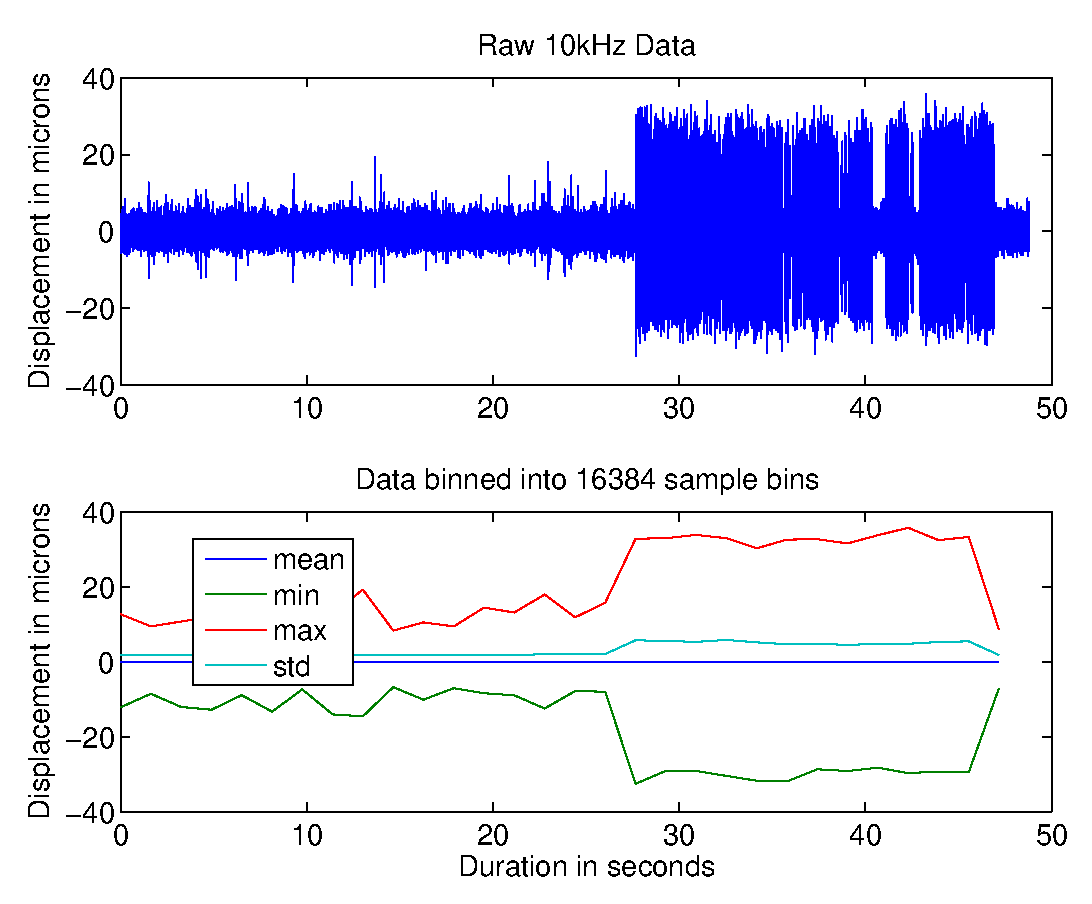
\includegraphics[width=.9\linewidth]{binning}
\end{center}
\end{frame}


% ------------------------------------------------------------------------------
%
\begin{frame}\frametitle{Archiver Services}

The FA archiver provides the following data over TCP/IP to any connecting
machine:

\begin{itemize}

\item Subscription to any subset of the complete CC data stream.
\note{If the client doesn't take data rapidly enough it will be disconnected by
the server.}

\item Subscription to any subset of the complete CC data stream decimated by
filtering by a factor of 10.

\item Access to any part of the historical archive, both full and decimated,
indexed by timestamp.

\end{itemize}
\end{frame}



% ------------------------------------------------------------------------------
%
\begin{frame}\frametitle{Spectrum Analysis Tool}
\begin{center}
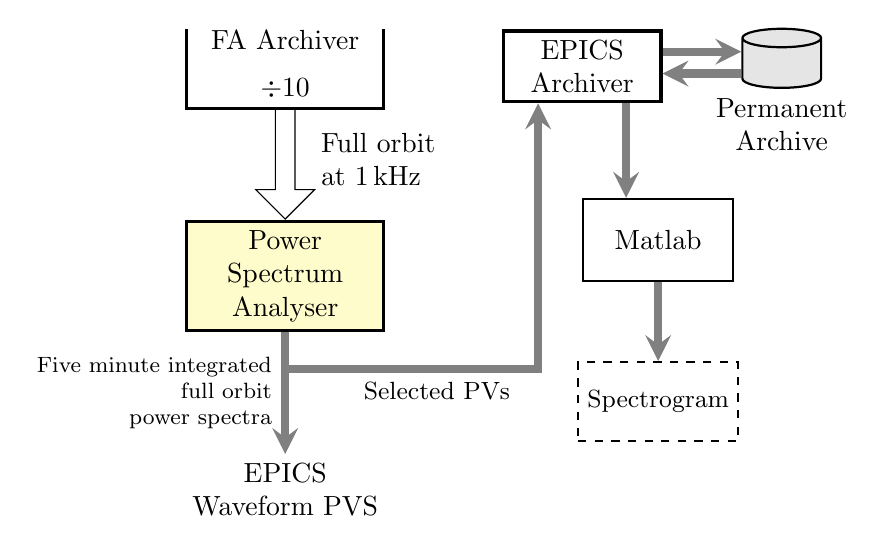
\begin{tikzpicture}

\draw [very thick]
    (0,0) coordinate(ar-nw) -- ++(0,-10mm) --
    ++(25mm,0) coordinate[midway] (ar-s) -- ++(0,10mm) coordinate(ar-ne);
\node [anchor=north, inner sep=0pt] at ($(ar-nw)!.5!(ar-ne)$) {FA Archiver};
\node [anchor=south] at (ar-s) {$\div 10$};

\node [draw, single arrow, rotate=-90, anchor=west, minimum height=14mm,
    label={[align=left, xshift=2mm]above:Full orbit\\at 1\,kHz}]
    (from-archiver) at (ar-s) {};
\node [draw, very thick, anchor=north, align=center, minimum width=25mm,
    fill=yellow!20]
    (analyser) at (from-archiver.east) {Power\\Spectrum\\Analyser};

\node [align=center] (pvs)
    at ($(analyser.south)+(0,-20mm)$) {EPICS\\Waveform PVS};
\draw [gray, line width=3pt, ->] (analyser) -- (pvs)
    coordinate[pos=0.3] (pv nw)
    node [anchor=east, pos=0.5, black, align=right, font=\footnotesize]
    {Five minute integrated\\full orbit\\power spectra};

\node [draw, very thick, align=center, anchor=north west, minimum width=20mm]
    (epics ar) at (40mm,0) {EPICS\\Archiver};
\node [disk icon, anchor=west, xshift=10mm, fill=black!10,
    label={[align=center]below:Permanent\\Archive}]
    (disk) at (epics ar.east) {};
\draw [gray, line width=3pt, ->] (disk.160 -| epics ar.east) -- (disk.160);
\draw [gray, line width=3pt, <-] (disk.190 -| epics ar.east) -- (disk.190);

\draw [gray, line width=3pt, ->] (pv nw) -| (epics ar.-140)
    node [pos=0.3, black, below, font=\small] {Selected PVs};


\node [draw, thick, anchor=north west, inner sep=4mm, yshift=-12mm]
    (matlab) at (epics ar.south) {Matlab};
\draw [gray, line width=3pt, ->]
    (epics ar.-40) -- (epics ar.-40 |- matlab.north);

\node [draw, thick, anchor=north, yshift=-10mm, font=\small, dashed,
    minimum height=10mm]
    (figure) at (matlab.south) {Spectrogram};
\draw [gray, line width=3pt, ->] (matlab) -- (figure);


\end{tikzpicture}

\end{center}
\end{frame}


% ------------------------------------------------------------------------------
%
\begin{frame}\frametitle{Spectrogram at one EBPM for a Week}
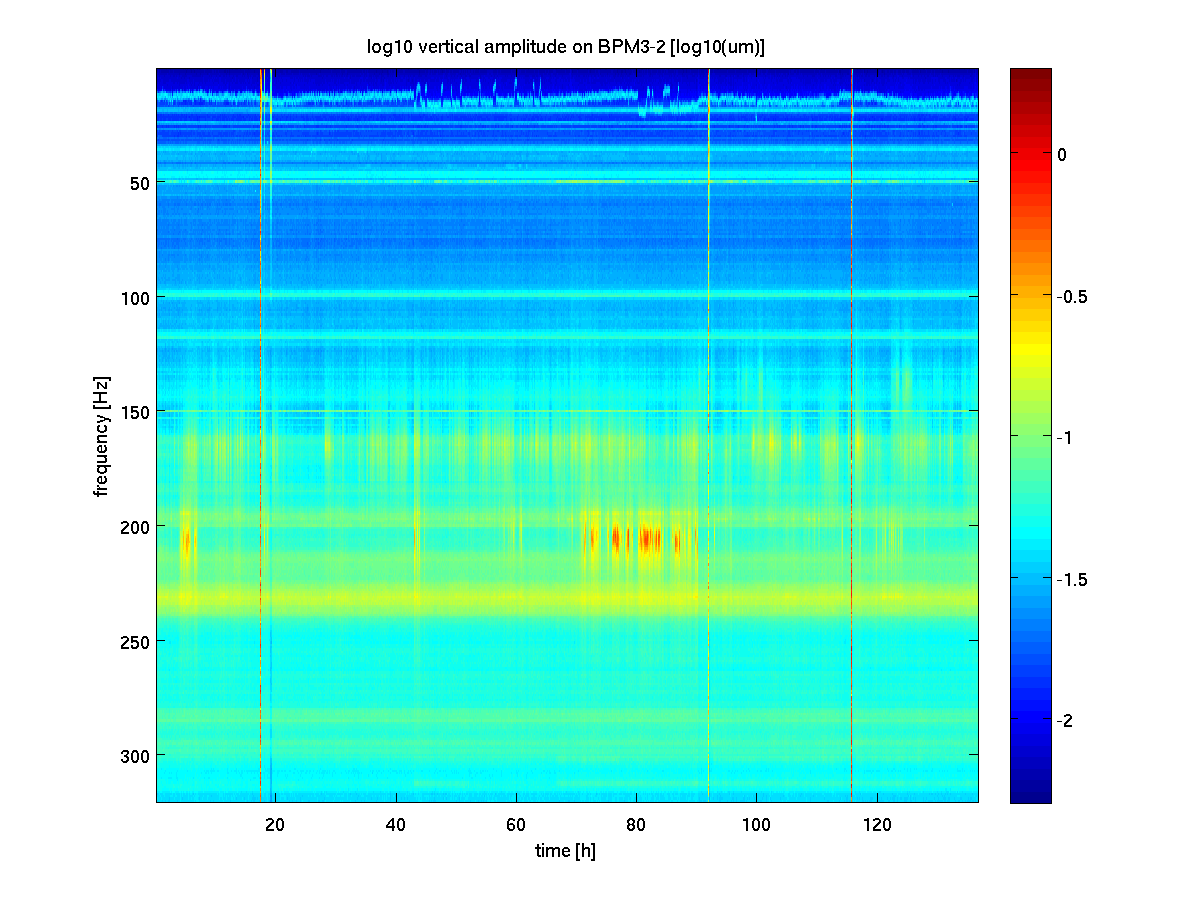
\includegraphics[width=\linewidth]{spectrogram-3-2}
\end{frame}



% ------------------------------------------------------------------------------
%
\begin{frame}\frametitle{FA Viewer}
\begin{center}
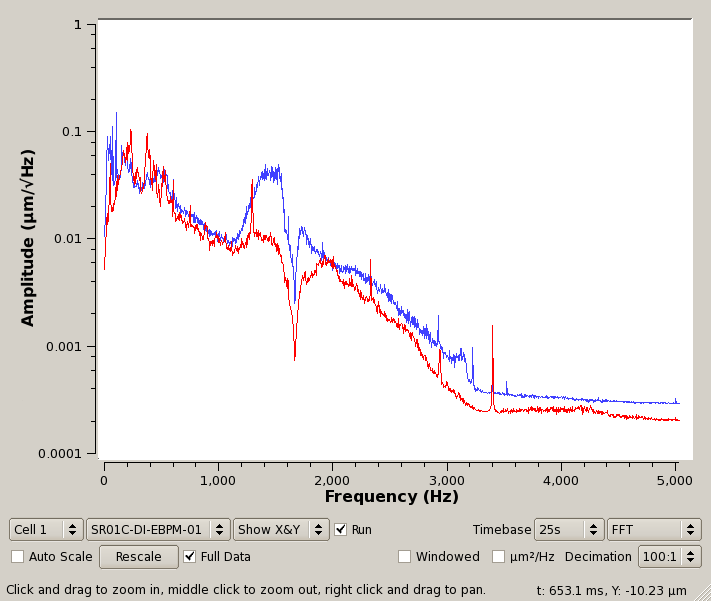
\includegraphics[width=.85\linewidth]{WEPMN004f6}
\end{center}
\end{frame}


% ------------------------------------------------------------------------------
%
\begin{frame}\frametitle{}


\end{frame}




% How to skip a block of (valid) code:
\iffalse \fi

\end{document}
